\section{Proposed System}

In this section, we describe our solution for providing privacy for prosumers without compromising the safety and security of the microgrid.
Figure~\ref{fig:softwareArchitecture} shows a high-level overview of the architecture of our solution.

\begin{figure}[h!]
\center
\begin{tikzpicture}[x=8cm, y=1.2cm,
  nodeStyle/.style={rounded corners=0.1cm, drop shadow={shadow xshift=0.05cm, shadow yshift=-0.05cm, fill=black}}
]
\draw [nodeStyle, fill=white]   (0, 0) rectangle    (1, 0.9) node [midway, align=center] {Communication network\\and operating system};

\draw [nodeStyle, fill=red!10]  (0, 1) rectangle    (1, 1.9) node [midway, align=center] {Communication anonymity\\(onion routing)};

\draw [nodeStyle, fill=blue!10] (0, 2) rectangle    (1, 2.9) node [midway, align=center] {Distributed ledger\\(blockchain)};

\draw [nodeStyle, fill=red!10]  (0,    3) rectangle (0.45, 3.9) node [midway, align=center] {Transaction anonymity\\(mixing service)};
\draw [nodeStyle, fill=blue!10] (0.47, 3) rectangle (0.72, 3.9) node [midway, align=center] {Bid storage};
\draw [nodeStyle, fill=red!10 ] (0.74, 3) rectangle (1,    3.9) node [midway, align=center] {Active\\smart meter};

\draw [nodeStyle, fill=red!10] (0,    4) rectangle (0.49, 4.9) node [midway, align=center] {Prosumer anonymous\\trading process};
\draw [nodeStyle, fill=blue!10] (0.51, 4) rectangle (1,    4.9) node [midway, align=center] {Microgrid\\controller};
\end{tikzpicture}
\caption{High-level architecture of the proposed solution. Components marked red are introduced to provide privacy in a safe and secure manner. Components marked in blue are typical elements of a decentralized transactive microgrid.}
\label{fig:softwareArchitecture}
\end{figure}

\begin{figure*}[h]
\center
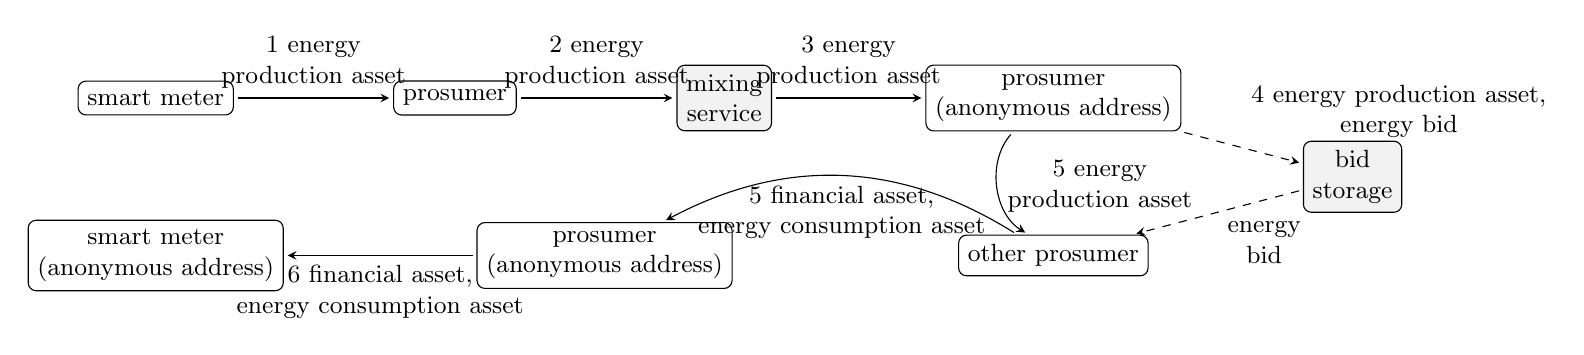
\begin{tikzpicture}[x=3.8cm, y=2cm, font=\small,
  system/.style={draw, align=center, rounded corners=0.1cm, fill=black!5},
  entity/.style={draw, align=center, rounded corners=0.1cm},
  asset/.style={midway, align=center},
  transfer/.style={->, >=stealth, shorten <=0.05cm, shorten >=0.05cm},
]
%\node[entity] (smartmeter) at (0.75, 0.5) {smart\\meter};
%\node[entity] (prosumer1) at (1.25, 1) {prosumer};
%\node[system] (mixing1) at (2, 1) {mixing\\service};
%\node[entity] (prosumer2) at (3, 1) {prosumer\\(alternative address)};
%\node[system] (bidstorage) at (4, 1) {bid\\storage};
%\node[entity] (partner) at (4, 0) {other prosumer};
%\node[entity] (prosumer3) at (3, 0) {prosumer\\(alternative address)};
%\node[system] (mixing2) at (2, 0) {mixing\\service};
%\node[entity] (prosumer4) at (1.25, 0) {prosumer};
\node[entity] (smartmeter) at (0, 1) {smart meter};
\node[entity] (prosumer1) at (1, 1) {prosumer};
\node[system] (mixing1) at (1.9, 1) {mixing\\service};
\node[entity] (prosumer2) at (3, 1) {prosumer\\(anonymous address)};
\node[system] (bidstorage) at (4, 0.5) {bid\\storage};
\node[entity] (partner) at (3, 0) {other prosumer};
\node[entity] (prosumer3) at (1.5, 0) {prosumer\\(anonymous address)};
\node[entity] (smartmeter2) at (0, 0) {smart meter\\(anonymous address)};

%\draw[transfer] (smartmeter) -- node [asset, above left] {energy\\production asset} (prosumer1);
%\draw[transfer] (prosumer1) -- node [asset, above] {energy\\production asset} (mixing1);
%\draw[transfer] (mixing1) -- node [asset, above] {energy\\production asset} (prosumer2);
%\draw[transfer, dashed] (prosumer2) -- node [asset, above] {energy production asset,\\energy bid} (bidstorage);
%\draw[transfer, dashed] (bidstorage) -- node [asset, right] {energy\\bid} (partner);
%\draw[transfer, bend right=15] (partner) to node [asset, below] {financial asset,\\energy\\consumption asset} (prosumer3);
%\draw[transfer, bend right=7.5] (prosumer2) to node [asset, above right] {energy\\prod. asset} (partner);
%\draw[transfer] (prosumer3) -- node [asset, below] {financial asset,\\
%energy consumption asset} (mixing2);
%\draw[transfer] (mixing2) -- node [asset, below] {financial asset,\\energy consumption asset} (prosumer4);
%\draw[transfer] (prosumer4) -- node [asset, below left] {financial\\asset} (smartmeter);

\draw[transfer] (smartmeter) -- node [asset, above] {\circled{1} energy\\production asset} (prosumer1);
\draw[transfer] (prosumer1) -- node [asset, above] {\circled{2} energy\\production asset} (mixing1);
\draw[transfer] (mixing1) -- node [asset, above] {\circled{3} energy\\production asset} (prosumer2);
\draw[transfer, dashed] (prosumer2) -- node [asset, above right] {\circled{4} energy production asset,\\energy bid} (bidstorage);
\draw[transfer, dashed] (bidstorage) -- node [asset, below right] {energy\\bid} (partner);
\draw[transfer, bend right=30] (partner) to node [asset, below] {\circled{5} financial asset,\\energy consumption asset} (prosumer3);
\draw[transfer, bend right=50] (prosumer2) to node [asset, right] {\circled{5} energy\\production asset} (partner);
\draw[transfer] (prosumer3) -- node [asset, below] {\circled{6} financial asset,\\
energy consumption asset} (smartmeter2);
\end{tikzpicture}
\caption{Simplified overview of the flow of assets from the perspective of a prosumer who sells energy. Note that in order to prevent de-anonymization, a prosumer should use multiple addresses and multiple rounds of mixing.}
\label{fig:sellFlow}
\end{figure*}

\subsection{Overview of the Trading Process}
We begin with a semi-formal description of the energy trading process from the prosumers' perspective.
In subsequent subsections, we will describe the assets, transactions, and services in our system in more detail.

First, consider a prosumer who would like to sell energy to another prosumer (this case is illustrated in Figure~\ref{fig:sellFlow}).
As its very first step, the prosumer obtains an \emph{energy production asset} from its smart meter.
An energy production asset represents a permission to sell a certain amount of energy, and it is used to enforce safety requirements.
If the prosumer has sufficient unsold production capacity, the smart meter creates and transfers a production asset to the prosumer using a \emph{smart meter transaction} \circled{1}, which is recorded on the distributed ledger.

At this point, the production asset can still be traced back to the prosumer since the ledger is public.
To achieve anonymity, the prosumer transfers the production asset to a \emph{mixing service} using an \emph{energy and financial transaction} \circled{2}, which is also recorded on the distributed ledger.
In turn, the mixing service transfers the production asset to an \emph{anonymous address} \circled{3}\todo{We should probably insert a good definition here for reader who are unfamiliar with blockchain transactions.}, which is randomly generated and controlled by the prosumer.
Since the mixing service transfers assets from multiple prosumers to multiple anonymous addresses at the same time, and the anonymous addresses were chosen at random by the prosumers, the assets cannot be traced back to the original prosumers after mixing.\footnote{Note that prosumers should divide their assets between multiple anonymous addresses; otherwise, each asset might be traced back to its prosumer based on the amount of energy that it contains.}

Now, the prosumer can engage in energy trading anonymously.
To find a trade partner, it can either post an \emph{energy bid} on the bid storage, or simply search the storage for an acceptable \emph{energy ask}.
To post an energy bid, the prosumer first proves to the storage service -- without revealing its original identity -- that it owns a production asset stored at an anonymous address.
It can then post the energy bid \circled{4}, which contains an anonymous communication address\footnote{We discuss communication anonymity later.}, a price, and a reference to the production asset.
If another prosumer, who would like to buy energy, finds the bid acceptable, it can contact the selling prosumer at the communication address given by the bid.

The seller and buyer can execute the trade by creating an energy and financial transaction together \circled{5}, and recording it on the ledger.
This transaction transfers the production asset from the seller to the buyer, and a \emph{financial asset} and an \emph{energy consumption asset} from the buyer to the seller.
A financial asset represents a certain amount of money, while a consumption asset represents a permission to buy a certain amount of energy, which is used to enforce safety requirements similarly to production assets.

Finally, the selling prosumer deposits the financial and consumption assets to its smart meter using an energy and financial transaction.
To ensure that the prosumer remains anonymous, it transfers the assets to an anonymous address that is randomly generated and controlled by the smart meter \circled{6}.
Once the smart meter has received the assets, it credits the financial amount to and deducts the energy amount from the prosumer, for billing purposes.
Note that in order to enforce safety requirements, the prosumer must always deposit the same amount of consumption assets as the amount of production assets obtained at the beginning; otherwise, unaccounted consumption assets might be used to trade excessive amounts.

Second, consider a prosumer who would like to buy energy from another prosumer.
Since the trading process is very similar to the case of the selling prosumer, we will discuss only the differences.
In the first step, the prosumer tries to obtain a financial asset and an energy consumption asset from its smart meter.
If the prosumer has the consumption capacity and good financial standing, the smart meter transfers the assets to the prosumer and adds the financial amount to the prosumer's bill.
After transferring the assets through a mixing service, the prosumer is ready to post an energy ask on the bid service.
To do so, it first proves the ownership of both the financial asset and the consumption asset to the service, and then posts the energy ask, which includes an anonymous communication address.
If a partner is found, the trade is executed as described before, the prosumer playing the role of the buyer.
Finally, the prosumer deposits the purchased energy production asset to the anonymous address of its smart meter,
which credits the energy amount to the prosumer, for billing purposes.
Note that if the prosumer has not used up the financial asset completely, then the remainder may also be deposited back to the smart meter.

\subsection{Timing}
The ability to specify points or intervals in time is crucial.
For example, control signals specify how the load should change at certain points in time, energy trades specify when energy will be consumed or produced, etc.
To facilitate processing signals and transactions, we divide time into fixed-length intervals, and specify points or periods in time using these discrete timesteps.
The length of the time interval is determined by mapping the timing assumptions of the power system to our platform.
%In our implementation, 
For example, the default length of the time interval may be 4 seconds, which corresponds to how frequently the control signal of the DSO typically changes.

\subsection{Transactions}

In the previous subsection, we gave an overview of how transactions are used in the trading process to transfer various assets.
Here, we detail the format of these transactions, and the rules that they have to satisfy to be valid and recorded on the ledger.
We also introduce and detail the format of regulatory transactions, which the DSO uses to regulate the microgrid.

\subsubsection{Timing}

The ability to specify points or intervals in time is crucial.
For example, control signals specify how the microgrid load should change at certain points in time, energy trades specify when energy will be consumed or produced, etc.
To facilitate processing signals and transactions, we divide time into fixed-length intervals, and specify points or periods in time using these discrete timesteps.
The length of the time interval is determined based on the timing assumptions of the physical power system.
For example, the default length of the time interval may be 4 seconds, which corresponds to how frequently the control signal of the DSO typically changes.
\Abhishek{We need to add citation here. I will add that tomorrow.}
\Abhishek{What about the deadline within which the transactions should finish? Do we need to say anything here?}
\Aron{Ideally, we should discuss the timing constraints of the ledger (probably when we introduce it), but we would first need to make space for this discussion.}

\subsubsection{Assets}

Before we can discuss transactions, we must define the format of three assets that these transactions may transfer.
First, an \emph{energy production asset} (EPA) is defined by
\begin{compactitem}
\item \field{power}: non-negative amount of power to produced (for example, measured in watts),
\item \field{start}: first time interval in which energy is to be produced,
\item \field{end}: last time interval in which energy is to be produced.
\end{compactitem}
Second, an \emph{energy consumption asset} (ECA) is defined by the same fields; however, for this asset, the fields define energy consumption instead of production.
Finally, a \emph{financial asset} (FA) is defined by a single non-negative number \field{amount}, which can be denominated in either a fiat currency (e.g., US dollars) or a cryptocurrency.

\subsubsection{Energy and Financial Transactions}

Energy and financial transactions transfer energy and financial assets from one address to another.
Prosumers use these transactions for multiple purposes: to trade energy by exchanging assets with other prosumers, to prove to the bid storage that they have production or consumption capacity, to hide their identity by transferring assets to and from mixing services, and to deposit assets at their smart meter.
%
An energy and financial transaction contains the following fields:
\begin{compactitem}
\item \field{EPA\_in}: list of EPA inputs, each of which is defined by
\begin{itemize}[leftmargin=0.5em,nosep]
\item \field{out}: reference to an EPA output of a previous transaction,
\item \field{sig}: signature for referenced output,
\end{itemize}
\item \field{ECA\_in}: list of ECA inputs, each of which is defined by
\begin{itemize}[leftmargin=0.5em,nosep]
\item \field{out}: reference to an ECA output of a previous transaction,
\item \field{sig}: signature for referenced output,
\end{itemize}
\item \field{FA\_in}: list of FA inputs, each of which is defined by
\begin{itemize}[leftmargin=0.5em,nosep]
\item \field{out}: reference to an FA output of a previous transaction,
\item \field{sig}: signature for referenced output,
\end{itemize}
\item \field{EPA\_out}: list of EPA outputs, each of which is defined by
\begin{itemize}[leftmargin=0.5em,nosep]
\item \field{EPA}: an energy production asset,
\item \field{address}: address to which EPA is transferred,
\end{itemize}
\item \field{ECA\_out}: list of ECA outputs, each of which is defined by
\begin{itemize}[leftmargin=0.5em,nosep]
\item \field{EPA}: an energy consumption asset,
\item \field{address}: address to which ECA is transferred,
\end{itemize}
\item \field{FA\_out}: list of FA outputs, each of which is defined by
\begin{itemize}[leftmargin=0.5em,nosep]
\item \field{EPA}: a financial asset,
\item \field{address}: address to which FA is transferred,
\end{itemize}
\end{compactitem}
This transaction transfers the assets specified in the input lists to the addresses specified in the output lists. 
Note that assets may be divided or combined, as the input and output lists may differ in length.

An energy and financial transaction is valid (and can be recorded on the ledger) if the following three conditions hold.
\begin{itemize}[noitemsep,topsep=-\parskip]
\item None of the outputs referenced by the inputs have been spent by a transaction that has been recorded on the ledger.
\item All of the signatures are valid, which ensures that only the current owner can transfer an asset.
\item For each asset type (and for each timestep), the sum of inputs and outputs is equal.
For example, in the case of energy production assets, the condition is
\begin{align*}
& \forall t: \sum_{\substack{out \,\in\, \field{EPA\_out}:\\out.\field{EPA}.\field{start} \leq t \leq out.\field{EPA}.\field{end}}} out.\field{EPA}.\field{power} \nonumber \\
& = \sum_{\substack{in \,\in\, \field{EPA\_in}:\\in.\field{out}.\field{EPA}.\field{start} \leq t \leq in.\field{out}.\field{EPA}.\field{end}}} in.\field{out}.\field{EPA}.\field{power}  .
%
%& \forall t: \sum_{out \in \field{EPA\_out}} out.\field{EPA}.\field{power} \cdot 1_{\left\{out.\field{EPA}.\field{start} \leq t \leq out.\field{EPA}.\field{end}\right\}} \nonumber \\
%& = \sum_{in \in \field{EPA\_in}} in.\field{out}.\field{EPA}.\field{power} \cdot 1_{\left\{in.\field{out}.\field{EPA}.\field{start} \leq t \leq in.\field{out}.\field{EPA}.\field{end}\right\}} ,
\end{align*}
%where $1_x$ is equal to $1$ if $x$ is true, and it is $0$ otherwise.
%\begin{equation}
%\forall t: \sum_{out \in \left\{out' \middle| out' \in \text{ EPA outputs} \wedge out'.EPA.start \leq t \leq out'.EPA.end\right\}} out.EPA.Power = \sum_{in \in \left\{in' \middle| in' \in \text{ EPA inputs} \wedge in'.EPA.start \leq t \leq in'.EPA.end\right\}} in.EPA.Power .
%\end{equation}
The conditions for consumption and financial assets can be described formally in similar ways.
\end{itemize}
%If a transaction submitted to the ledger is valid, it will be permanently recorded.

\subsubsection{Smart-Meter Transactions}

Prosumers use smart-meter transactions to withdraw energy and financial assets from their own smart meters, before they engage in trading.
%
A transaction contains the following fields:
\begin{compactitem}
\item \field{EPA\_out}: list of EPA outputs (see above),
\item \field{ECA\_out}: list of ECA outputs (see above),
\item \field{FA\_out}: list of FA outputs (see above),
\item \field{id}: smart meter's identifier,
\item \field{sig}: smart meter's signature over the transaction.
\end{compactitem}
This transaction creates and transfers the assets to the prosumer's addresses, which are specified in the output lists.

The smart meter signs the transaction only if the prosumer is allowed to withdraw these assets.
More specifically, the amount of withdrawn assets can never exceed certain limits that are set by the DSO.
For example, in the case of EPA, the following condition must be satisfied for prosumer $i$:
\begin{equation}
\forall t: \sum_{tr \,\in\, \field{TR}_i} \sum_{\substack{out \,\in\, tr.\field{EPA\_out}:\\out.\field{EPA}.\field{start} \leq t \leq out.\field{EPA}.\field{end}}} out.\field{EPA}.\field{power} < \field{MAXEPA}_i ,
\end{equation}
where $\field{TR}_i$ is the set of smart-meter transactions recorded for prosumer $i$ and $\field{MAXEPA}_i$ is the withdrawal limit.
The condition for consumption assets is similar, based on a limit $\field{MAXECA}_i$.
For financial assets, the smart meter takes into account the amounts withdrawn and deposited, as well as the outside bill payments to the DSO.

\Aron{To address malfunctioning or compromised smart meters, we could also impose a limit on withdrawals.}
A transaction is valid if the following two conditions hold.
\begin{itemize}[noitemsep,topsep=-\parskip]
\item The smart meter identified in the transaction has been authorized by a regulatory transaction that was previously recorded on the ledger.
\item The smart meter's signature is valid (for public key, see regulatory transactions).
\end{itemize}

\subsubsection{Regulatory Transactions}

The DSO uses regulatory transactions for two purposes: to manage the set of authorized smart meters and to change the price policy.
%First, to change the set of smart meters that are authorized to sign transactions, the DSO authorizes or bans individual smart meters.
First, whenever a new smart meter is installed, the DSO notifies the microgrid by authorizing the device using a regulatory transaction.
Similarly, whenever a smart meter is deactivated (e.g., because service is stopped or the device is believed to be malfunctioning or compromised), the DSO notifies the microgrid by banning the device.
Second, to influence microgrid load, the DSO can set a price policy, which includes a price at which prosumer may buy energy from the DSO and a price at which they may sell energy to the DSO.

A regulatory transactions contain the following fields:
\begin{compactitem}
\item \field{authorize}: list of smart meters to be authorized, each of which is defined by
\begin{compactitem}
\item \field{id}: identifier of the smart meter,
\item \field{pubkey}: public key of the smart meter,
\end{compactitem}
\item \field{ban}: list of identifiers of smart meters to be banned, 
\item \field{priceConsumption}: price at which DSO sells energy,
\item \field{priceProduction}: price at which DSO buys energy,
\item \field{time}: timestep after which authorizations, bans, and price changes should take effect,
\item \field{sig}: DSO's signature over the transaction.
\end{compactitem}

A regulatory transaction of this type is valid if %the following two conditions hold:
%\begin{compactitem}
%\item 
\field{timestep} is not in the past and % specified in the transaction is in the future.
%\item 
the DSO's signature is valid.
%\end{compactitem}
%
The active prices for timestep $t$ are given by the last regulatory transaction recorded on the ledger whose \field{time} is less than $t$.
Similarly, regulatory transactions that are recorded on the ledger later override the authorizations and bans of earlier transactions.



\subsection{Services}

In this subsection, we describe the various services that are implemented in our system. %on which transactions are built and which build on transactions.
We have already discussed the distributed ledger, which permanently stores valid transactions.
Now, we will introduce anonymous communication service, mixing service for transaction anonymity, anonymous bid storage, and smart-meter based billing.\Aron{Revise list based on final organization!}

\subsubsection{Communication Anonymity}
Firstly, we must provide an anonymous communication layer, on which we can build all the other services in our system.
Without this communication layer, transactions and bids could be easily de-anonymized based on their sources' network identifiers (e.g., IP or MAC addresses).

We can employ well-known and widely used techniques for anonymous communication, such as \emph{onion routing}~\cite{reed1998anonymous}.
To build an onion network, the smart meters, prosumers, and other devices can act as onion routers, and the list of onion routers in a microgrid can be published on the ledger.
In practice, this service can built on 
%In our first implementation, we can use
 the free and open-source Tor software with private Directory Authorities.
In this case, anonymous communication addresses in bids and asks correspond to public-keys that identify Tor hidden services.
% ritter.vg: "run your own tor network"
% https://ritter.vg/blog-run_your_own_tor_network.html

\subsubsection{Transaction Anonymity}
Communication anonymity is necessary for anonymous trading, but it is not sufficient: if prosumers used their own accounts to transfer assets, trades would not be anonymous.
Fortunately, most distributed ledgers allow users to easily generate new addresses\footnote{The usage of the term \emph{address} varies between distributed ledgers, but our system could be implemented using any popular ledger, such as Bitcoin and Ethereum. 
Specifically, we use the term address to denote a possible destination for asset transfers. 
Assets transferred to an address can be used only by someone who knows the private key of the address (typically, the one who generated the address).} 
at random.
Since these addresses are generated randomly, they are anonymous in the sense that no one can tell who generated them.
However, if prosumers simply transferred assets to these addresses, they could be easily de-anonymized by tracing the assets back to the prosumers.

To prevent this, prosumers transfer assets to their anonymous addresses through a \emph{mixing service}. 
The mixing service prevents tracing the assets back to their original owners by mixing together multiple incoming transfers and multiple outgoing transfers, thereby hiding the connections between the prosumers and the anonymous addresses.
In practice, a mixing service can be implemented using multiple approaches.
The simplest one is to use a \emph{trusted third party}, called a cryptocurrency tumbler, which can receive and send assets.
However, anonymity in this case depends on the trustworthiness and reliability of the third party, who could easily de-anonymize the addresses.
A more secure approach is to used decentralized protocols, such as CoinShuffle~\cite{ruffing2014coinshuffle} or Xim~\cite{bissias2014sybil}.
These protocols enable participants to mix assets with each other, thereby eliminating the need for a trusted third party, which would constitute a single point of failure.
Some newer cryptocurrencies, such as Zerocoin~\cite{miers2013zerocoin},  provide built-in mixing services, which are often based on cryptographic principles and proofs.

\begin{comment}
We must provide prosumers with the ability to create and publish transactions anonymously.
More specifically, prosumers should be able to purchase or sell energy without revealing their identity; however, these transaction must also be verifiable and enforceable.

We may achieve this goal using multiple approaches for blockchain transaction anonymity:
\begin{itemize}
\item Mixing services (also known as tumblers) mix potentially identifiable assets on a blockchain with others, thereby preventing tracing individual assets back to their original source. 
In our case, assets to be mixed include virtual balances of fiat currencies as well as energy production and consumption.
\item Cryptographic anonymity for transactions is provided, for example, by Zerocoin~\cite{miers2013zerocoin}. Similarly to mixing service, Zerocoin can prevent tracing assets on a blockchain.
\end{itemize}
Using the above techniques, we can enable prosumers to trade energy anonymously (i.e., without revealing their true identities), but at the same time prevent them from altering their energy or financial balances without a valid transaction.

However, we must also ensure that 1) smart meters know the amount of energy purchased or sold by their prosumer and 2) prosumers cannot purchase or sell more energy than their capacity.
To satisfy both of these constraints, all energy trades must start with the prosumer withdrawing a certain amount of energy production or consumption from its smart meter:
\begin{itemize}
\item If a prosumer wishes to sell energy, it must first withdraw an energy asset from its smart meter using a blockchain transaction.
This transaction must be signed by the smart meter, which enables the smart meter to 1) keep track of the amount of energy traded by the prosumer as well as to 2) enforce safety requirements by limiting the amount of energy that can be withdrawn.
\item If a prosumer wishes to buy energy, it must first withdraw an energy consumption asset from its smart meter in a way similar to withdrawing an energy production asset.
\end{itemize}
\end{comment}

\subsubsection{Bidding Anonymity}
Finally, we must provide prosumers with the ability to post energy bids and asks anonymously.
To this end, we create a storage for anonymous bids that is readable by all the prosumers in the microgrid.
Any prosumer may submit a bid to this storage; however, in order to do so, they must provide a zero-knowledge proof of owning the assets that are to be traded:
\begin{itemize}
\item To submit an energy sell bid, the prosumer must prove that it owns an energy production asset on the chain.
\item To submit an energy buy bid, the prosumer must prove that it own an energy consumption asset as well as financial assets on the chain.
\end{itemize}

\subsubsection{Billing}

The energy consumption balance $E_i^t$ of prosumer $i$ in timeslot~$t$ is
\begin{align*}
E_i^t = & \hphantom{+} \text{measured consumption} - \text{measured production} \\
 & + \text{EPA deposited by $i$} - \text{EPA withdrawn by $i$} .
\end{align*}
Notice that energy consumption assets are not necessary for billing, they are only used to enforce safety requirements.

The financial balance $F_i^t$ of prosumer $i$ in timeslot $t$, which is to be paid by the prosumer to the DSO, is
\begin{align*}
F_i^t = & \hphantom{+} \text{FA deposited by $i$ in $t$} - \text{FA withdrawn by $i$ in $t$} \\
 & + \begin{cases}
E_i^t \cdot \field{priceProduction} & \text{ if } E_i^t < 0 \\
- E_i^t \cdot \field{priceConsumption} & \text{ otherwise.} 
\end{cases}
\end{align*}

\TODO{discussion of microgrid control based on bids and trades? (update subsubsection title)}



